\documentclass[tikz,border=5pt]{standalone}
\usepackage{graphicx}
\usepackage{comment}
\usepackage{xcolor}
\usetikzlibrary{matrix,positioning}

\usepackage[scaled=0.95]{helvet}
\renewcommand\familydefault{\sfdefault}
\usepackage{sansmath}
\sansmath


\begin{document}

    \centering
	\definecolor{Mycolor1}{HTML}{1F77B4}
	\definecolor{Mycolor2}{HTML}{FF7F0E}
	\definecolor{Mycolor3}{HTML}{2CA02C}
	\definecolor{Mycolor4}{HTML}{D62728}
	\definecolor{Mycolor5}{HTML}{9467BD}

% From (0.977995, 0.861432, 0.142808)
\definecolor{colorA}{HTML}{F9DC24}

% From (0.933232, 0.482780, 0.319325)
\definecolor{colorB}{HTML}{EE7B51}

% From (0.050383, 0.029803, 0.527975)
\definecolor{colorC}{HTML}{0D0887}

% From (0.714883, 0.187299, 0.546338)
\definecolor{colorD}{HTML}{B6308B}

% From (0.356359, 0.003798, 0.647810)
\definecolor{colorE}{HTML}{5B01A5}



\definecolor{pltGreen}{rgb}{0.0, 0.5019607843137255, 0.0}
\definecolor{pltRed}{rgb}{1.0, 0.0, 0.0}

\begin{tikzpicture}[every node/.style={inner sep=0, outer sep=0}]

  %%=== Top matrix: Full Model Fit ===%%
  \matrix (top) [
    matrix of nodes,
    name=top,
    column sep=1em, row sep=1em,
    nodes={anchor=center}
  ] {
    %Title
    % \node[text width=0.9\textwidth, align=center]
    %   {\large\sffamily Full Model Fit}; & 
    % \\
    \node[name=top-1-1, xshift=0.0cm]{
      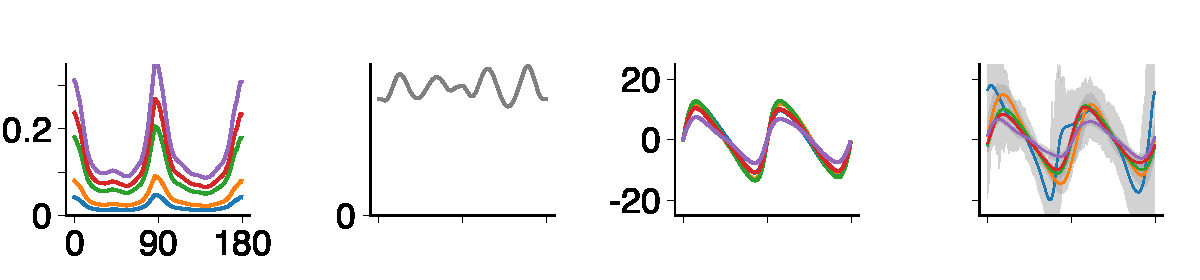
\includegraphics[width=0.6\textwidth]
        {figures/RunGardelle_FreePrior_CosineLoss_VIZFig7.py_8_0_10.0_180.pdf}
    }; \\
    % Legend
    \node{
\scriptsize
Exposure:\quad
\textcolor{Mycolor1}{\rule[0.5ex]{1em}{1pt}}\,20 ms\quad
\textcolor{Mycolor2}{\rule[0.5ex]{1em}{1pt}}\,40 ms\quad
\textcolor{Mycolor3}{\rule[0.5ex]{1em}{1pt}}\,80 ms\quad 
\textcolor{Mycolor4}{\rule[0.5ex]{1em}{1pt}}\,160 ms\quad
\textcolor{Mycolor5}{\rule[0.5ex]{1em}{1pt}}\,1000 ms
    }; & 
    \\
  };
 \node[above=0mm of top-1-1, xshift=-2.7cm, yshift=-0.15cm]{   \footnotesize \shortstack{Resources}}; 
 \node[above=0mm of top-1-1, xshift=-0.8cm, yshift=-0.15cm]{   \footnotesize \shortstack{Prior}}; 
 \node[above=0mm of top-1-1, xshift=1cm, yshift=-0.25cm]{   \footnotesize \shortstack{Bias \\ (Model)}}; 
 \node[above=0mm of top-1-1, xshift=2.9cm, yshift=-0.25cm]{   \footnotesize \shortstack{Bias \\ (Data)}}; 

  %%=== Bottom matrix: Identifying Loss Function ===%%
  \matrix (bot) [
    matrix of nodes,
    name=bot,
    below=2em of top.south west,
    anchor=north west,
    column sep=1em, row sep=1em,
    nodes={anchor=center}
  ] {
    % column labels
    \node[name=bot-1-1, xshift=0.026\textwidth]{\footnotesize\shortstack{1 level,\\1K trials}}; &
 \node[name=bot-1-2, xshift=0.026\textwidth]{   \footnotesize\shortstack{2 levels,\\ 1K trials}}; &
 \node[name=bot-1-3, xshift=0.026\textwidth]{   \footnotesize\shortstack{5 levels,\\ all trials}}; \\[-.9ex]
    % first row of plots
    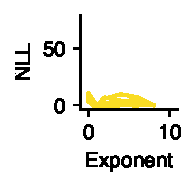
\includegraphics[width=0.18\textwidth]
      {figures/evaluateCrossValidationResults_Gardelle_180_Downsampled_TargetSize_Individual_ByFI.py_subplot_0_0.pdf} &
    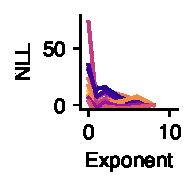
\includegraphics[width=0.18\textwidth]
      {figures/evaluateCrossValidationResults_Gardelle_180_Downsampled_TargetSize_Individual_ByFI.py_subplot_1_0.pdf} &
  %  \includegraphics[width=0.18\textwidth]
  %    {figures/evaluateCrossValidationResults_Gardelle_180_Downsampled_TargetSize_Individual_ByFI.py_subplot_2_1.pdf} 
    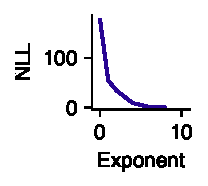
\includegraphics[width=0.18\textwidth]
      {figures/evaluateCrossValidationResults_Gardelle_180_Downsampled_TargetSize_Individual_ByFI.py_subplot_2_4.pdf} \\[1ex]
    % second row labels
 \node[name=bot-2-1, xshift=0.026\textwidth]{   \footnotesize \shortstack{1 level,\\ 2K trials}}; &
 \node[name=bot-2-2, xshift=0.026\textwidth]{   \footnotesize \shortstack{2 levels,\\ 2K trials}}; &
    {} \\[-.9ex]
    % second row of plots
    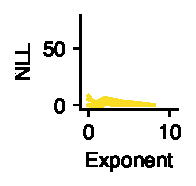
\includegraphics[width=0.18\textwidth]
      {figures/evaluateCrossValidationResults_Gardelle_180_Downsampled_TargetSize_Individual_ByFI.py_subplot_0_1.pdf} &
    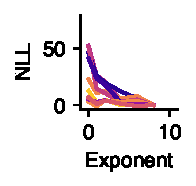
\includegraphics[width=0.18\textwidth]
      {figures/evaluateCrossValidationResults_Gardelle_180_Downsampled_TargetSize_Individual_ByFI.py_subplot_1_1.pdf} &
    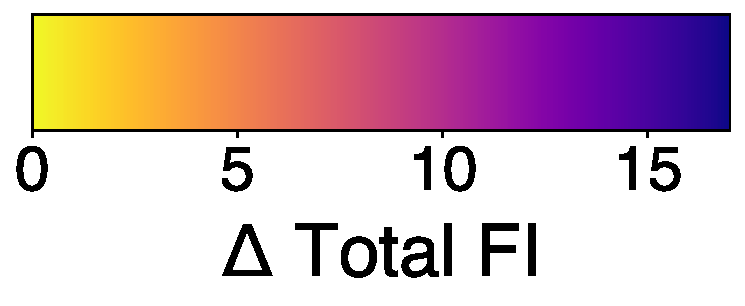
\includegraphics[width=0.18\textwidth]{figures/colorLegendFigure7_ByFI.py.pdf}\\
  };

% Top row labels
\node[anchor=north west, font=\sffamily] at ([xshift=0em,yshift=0.8em]top-1-1.north west) {a};
\node[anchor=north west, font=\sffamily] at ([xshift=5.5em,yshift=0.8em]top-1-1.north west) {b};
\node[anchor=north west, font=\sffamily] at ([xshift=11em,yshift=0.8em]top-1-1.north west) {c};
\node[anchor=north west, font=\sffamily] at ([xshift=16.5em,yshift=0.8em]top-1-1.north west) {d};

% Bottom matrix
\node[anchor=north west, font=\sffamily] at ([xshift=-1.4em,yshift=0.1em]bot-1-1.north west) {e};
\node[anchor=north west, font=\sffamily] at ([xshift=-1.4em,yshift=0.1em]bot-1-2.north west) {g};
\node[anchor=north west, font=\sffamily] at ([xshift=-1.4em,yshift=0.1em]bot-1-3.north west) {i};

\node[anchor=north west, font=\sffamily] at ([xshift=-1.4em,yshift=0.1em]bot-2-1.north west) {f};
\node[anchor=north west, font=\sffamily] at ([xshift=-1.4em,yshift=0.1em]bot-2-2.north west) {h};


  % Separate title node for the bottom grid
  % \node[
  %   font=\bfseries,
  %   above=1ex of bot.north
  % ] {Identifying Loss Function};

\end{tikzpicture}

%\textcolor{red}{need to double-check Total FI}

\begin{comment}
python3 RunGardelle_FreePrior_CosineLoss_VIZFig7.py 8 0 10.0 180
python3 evaluateCrossValidationResults_Gardelle_180_Downsampled_TargetSize_Individual_ByFI.py
\end{comment}
\end{document}

